\documentclass[10pt,twocolumn]{article}
\usepackage[margin=1in]{geometry}
\usepackage{amssymb}
\usepackage{color}
\usepackage{alltt}
\usepackage{fancybox}
\usepackage{graphicx}
\usepackage{framed}
\usepackage{enumitem} % For resuming enums
\usepackage{eso-pic}
\usepackage{verbatim} % adds environment for commenting out blocks of text & for better verbatim
\usepackage{etoolbox} % for conditional toggles
\usepackage[title,titletoc,toc]{appendix}
\geometry{a4paper}
\graphicspath{{../../imgs/}}
\title{\textbf{Patchistory}}
\newif\iforiginal
\newtoggle{original-rules}
\togglefalse{original-rules}
\iftoggle{original-rules}{
\originaltrue
}{
\originalfalse
}
\author{Jun-Hyup Kim \& Yeon-Min Jung}
\iftoggle{original-rules}{
\date{v1.3d 2014-11-10}
}{
\date{v1.3sk 2014-11-10}
}
\begin{document}
\definecolor{TFFrameColor}{gray}{0.5}
\definecolor{TFTitleColor}{gray}{1}
\newenvironment{BoxExample}%
{\begin{titled-frame}{Example}\noindent\ignorespaces}%
{\par\noindent\ignorespacesafterend\end{titled-frame}}
\newcommand\statExplain[2]{\begin{framed}{\noindent\textit{ #1 = #2}}\end{framed}}
\newcommand\eraCost[3]{[#1/#2/#3]}
\newcommand\myAction[1]{\texttt{#1}}
\newcommand\myPhase[1]{\textit{#1}}
\iftoggle{original-rules}{
\newcommand\victorypoint{Victory Point}
\newcommand\victorypoints{Victory Points}
\newcommand\vp{VP}
\newcommand\vps{VPs}
\newcommand\mineral{Mineral}
\newcommand\minerals{Minerals}
\newcommand\money{Money}
\newcommand\good{Resource}
\newcommand\goodss{Resource}
\newcommand\goods{Resources}
\newcommand\polf{Political Favour}
\newcommand\polfs{Political Favours}
\newcommand\baseland{Baseland}
\newcommand\baselands{Baselands}
\newcommand\psb{Player Status Board}
}{
\newcommand\victorypoint{Culture}
\newcommand\victorypoints{Culture}
\newcommand\vp{Culture}
\newcommand\vps{Culture}
\newcommand\mineral{Resource}
\newcommand\minerals{Resources}
\newcommand\money{Coin}
\newcommand\good{Good}
\newcommand\goodss{Goods}
\newcommand\goods{Goods}
\newcommand\polf{Political Point}
\newcommand\polfs{Political Points}
\newcommand\baseland{Capital Tile}
\newcommand\baselands{Capital Tiles}
\newcommand\psb{Reference Board}
}
\newcommand\tra{Transport Level (TRA)}
\newcommand\mil{Military Force (MIL)}
\newcommand\pol{Political Influence (POL)}
\newcommand\inlineImage[2][\linewidth]{\centerline{\includegraphics[width=#1]{../../imgs/#2.jpg}}}
\newcommand\actionCost[2]{#1 (#2):}
\newcommand\compHead[1]{\subsection*{#1}}
\newcommand\floatingImage[3][\linewidth]{\begin{figure}\centering\includegraphics[width=#1]{../../imgs/#3.jpg}\caption{#2}\end{figure}}
\maketitle
\tableofcontents
\section{Game Story}
\iforiginal
The mankind has evolved consistently over the great moments, and that great moments have been recorded through history.
\begin{verbatim}We start a new record.
We go back to those great moments,
and choose the future of our own.
We patch the history with new pieces
of events of our own choices.\end{verbatim}
Your country may have great men like Aristotle or Gandhi, or the grand monuments such as Pyramid and Eiffel Tower. Record your own history and build a kingdom greater than any other's, with Patchistory.
\else
Our history has been forged in great moments. Those moments are told and retold for generations, creating a record of our struggles, our joys.
\begin{verbatim}Now we begin a new record.
We return to those great moments,
and create a new history.
We will patch a new tapestry of events
to forge a history of our choosing.\end{verbatim}
Your civilisation may give rise to countless heroes such as Aristotle, Gandhi or Elizabeth I. You may construct dazzling Wonders like the Hanging Gardens, the Eiffel Tower, the Great Wall of China or many others.
Create your own history and build the greatest civilisation our world has ever seen in - Patchistory.
\fi
\section{Objective}
Across three Eras, the players will develop their nations. The development and prosperity of their country will be represented by \victorypoints. At the end of Era III, the player with the most \victorypoints\ will be declared the winner.
\section{Components}
\section{Component Overview}
\compHead{\baselands}
\inlineImage{Baselands}
Each \baseland\ has two sides, Liberty (easier) and Equality (harder). The Liberty side is indicated by a small ``L'' icon and the Equality side by a small ``E'' icon. Select one of the two \baselands\ to start the game. You should not mix the \baseland\ types within a single game.

On the Liberty side, each player will have a different starting arrangement and 2 workers will be placed after the initial auction. On the Equality side, each player will have the same starting arrangement and 1 worker will be placed after the initial auction.
\compHead{Icons}
\inlineImage{Icons}

\compHead{Player Screen}
\inlineImage{PlayerScreen}
Player Screens are used to hide your \goods, \vps\ and \money\ during the game. The Player Screen also contains a quick reference to the costs and rewards of war, the maintenance costs paid during the \myPhase{Maintain Heroes \& Wonders} phase and the actions that can be taken during the \myPhase{Diplomacy \& Management} phase.
\compHead{\psb}
\inlineImage{PlayerStatusBoard}
The \psb\ is divided into three sections. On the left is the descendants section where you will place your workers until they are born. This will also show the maintenance cost you must pay for your workers.

In the middle is a status track used to show your current Military Force, Political Influence and Transport Level.

On the right is the production track used to track your overall production of \minerals, Food, \vps\ and \money.

The status and production tracks are not intended to imply upper bounds, if you would run off the end of the track, use some mechanism to indicate that you have wrapped round. The \psb\ should be placed in front of the Player Screen, visible to the other players.
\compHead{Land Cards}
\inlineImage{LandCards}
Both sides of the Land Cards are used during the game. One side will have a white era icon (hereafter referred to as the White Side) and one side will have a black era icon (hereafter referred to as the Black Side).

On the White side you will find the coloured, General Buildings, some of which will have Activity Boxes (indicated by a golden frame). On the Black Side you will find the white-coloured Special Buildings along with Heroes and Wonders.

Land Cards are divided up into one or more Rooms of varying sizes. A Room which occupies one quarter of a Land Card is the most basic unit of size and is referred to as a 1x1 room. Each Room may hold at most one worker.
\compHead{Trade Routes}
\inlineImage{GeneralTradeRoute}
\inlineImage{AlliedTradeRoute}
Trade Routes represent connections between different Kingdoms. Through Trade Routes you can either peacefully gain \goods\ and negotiate alliances or aggressively threaten or go to war with your opponents. When placing a General Trade Route, ensure that the ``Start'' space faces the Kingdom of the player placing the route. There may be any number of General Trade Routes between any two Kingdoms.

Allied Trade Routes represent a strong Alliance between two Kingdoms. Once an Alliance is established, neither Kingdom may take any aggressive action (e.g. War or Threatening) without first breaking the Alliance. There can only be a single Allied Trade Route between any pair of Kingdoms.
\compHead{Status Markers}
\inlineImage{StatusMarkers}
These markers are placed on the tracks of your \psb\ to track the overall status of your Kingdom.
\compHead{Prosperity Cards}
\inlineImage{ProsperityCards}
Prosperity Cards are played during the \myPhase{Vote} phase at the end of each era. The cards will reward players for their relative standings in either the production levels of a specific \good\ or their capacity (i.e. number) of a particular room type. There are a total of 15 cards covering different \goods\ and room types.
\compHead{First Player Marker}
\inlineImage[2.5cm]{FirstPlayer}
Marks the First Player in each round. All other players must refer to the holder as ``King'' or ``Queen'' as appropriate. The First Player Marker is passed clockwise at the end of each round.
\compHead{Workers}
%\inlineImage{worker}
8 workers per player colour.
\compHead{\goodss\ Cubes}
\inlineImage{Resources}
Each \good\ is represented by a particular colour of wooden cube. Each colour comes in two sizes: small representing 1 unit of that \good; and large, representing 3 units of that \good.
\compHead{Round \& Phase Tokens}
\inlineImage[4cm]{RoundPhaseTokens}
These are placed on the Timeline Board to indicate which round and phase of the game the players are currently executing.
\compHead{Construction Tiles}
\centerline{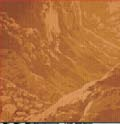
\includegraphics[height=1.25cm]{CT1}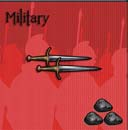
\includegraphics[height=1.25cm]{CT2}  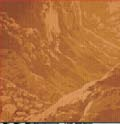
\includegraphics[height=1.25cm]{CT3}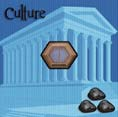
\includegraphics[height=1.25cm]{CT4}}
Construction tiles have Wasteland spaces on one side and General Buildings on the other. These are used when reclaiming spaces (replacing them with wasteland) or constructing new buildings. They are the size of a 1x1 Room.
\compHead{\money}
\centerline{
\includegraphics[width=1.25cm]{1Money}  
\includegraphics[width=1.25cm]{2Money}  
\includegraphics[width=1.25cm]{5Money}}
The coins represent \money\ and come in three denominations: 1, 2, and 5.
\compHead{\victorypoint\ Tokens}
\inlineImage[5cm]{VPTokens}
These tokens represent \victorypoints\ and come in five denominations: 1, 5, 10, 20 and 80.
\compHead{Auction Tokens}
\centerline{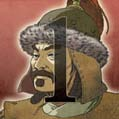
\includegraphics[height=1.25cm]{AT1}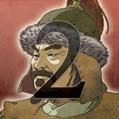
\includegraphics[height=1.25cm]{AT2}  
\includegraphics[height=1.25cm]{AT3}
\includegraphics[height=1.25cm]{AT4}}
These tokens are used during the auction phase in the two-player game. The red tokens feature Genghis Khan while the Blue tokens feature Rommel.
\compHead{Timeline Board}
\begin{tabular}{p{2cm} p{5cm}}
	\vspace{0pt}
	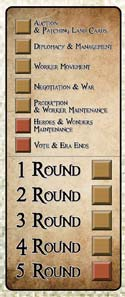
\includegraphics[width=2cm]{TimelineBoard}
	&
	\vspace{0pt}
The Timeline Board indicates the current round and which phase of the game is currently being played.
\end{tabular}
\section{Initial Setup}
\begin{itemize}
\item If playing with Liberty \baselands, each player randomly chooses a \baseland\ to start with.
\item Each player takes a Player Screen, a \psb\ and the 8 worker pieces of the same colour.
\item Each player places their 8 workers on the descendants section on the left hand side of their \psb.
\item Each player takes one of each of the seven different status markers and marks their current production levels on their \psb\ according to their \baseland.
\item Each player takes: 4 Food, 3 \money, 4 Random Construction Tiles and 20 \vps. These are all placed behind their Player Screen.
\item Each player receives 3 random Prosperity cards.
\item In a 3 or 4 player game, each player constructs a General Trade Route between their kingdom and the kingdom of the player to their left. In a 2 player game, no initial Trade Routes are placed.
\item The remaining General Trade Routes are placed near the play area in the Public Storage.
\item The remaining Construction Tiles are placed Wasteland-side up and shuffled.
\item The Land Cards should be sorted by Era, and the deck for each Era should be shuffled well.
\item The remaining \goods\ should be placed near the play area in a Public Storage.
\item The starting player will be the one who has most recently played a civilization game.
\end{itemize}
\begin{BoxExample}Given the \baseland\ shown below, the player should set up his \psb\ as shown. 8 workers are placed on the Descendants track. 4 Food, 3 \money, 20 \vps\ and 4 Construction Tiles are placed behind the Player Screen. Finally one General Trade Route is placed facing the Kingdom on the left in a 3 or 4 player game.\end{BoxExample}
\section{Game Overview}
The game is played across three Eras and each Era consists of five Rounds. During each Round, the following phases will be carried out in order:
\begin{enumerate}
\item Auction \& Patching Land Cards
\item Diplomacy \& Management (Domestic Politics)
\item Movement
\item Negotiation \& War
\item Production \& Maintain Workers
\end{enumerate}
In addition, the following three phases will be carried out at the end of the fifth round of each Era (i.e. three times during the game):
\begin{enumerate}[resume]
\item Maintain Heroes \& Wonders
\item Vote
\item End of an Era
\end{enumerate}

The game ends after the \myPhase{End of an Era} phase in Era III.

\subsection{General Rules}
\begin{itemize}
\item The tracks on the \psb\ are one of the most important pieces of information in the game. Their position will mostly change during the \myPhase{Patching Land Cards} and \myPhase{Movement} phases. Players should make every effort to ensure they are accurate and up to date at all times.

\item All tokens (\goods, \money, \vps, Construction Tiles) should be kept behind the Player Screens at all times.
\iftoggle{original-rules}{
\item A player may not have fewer than 0 \vps.
}{
\item A player may not have less than 0 \vps.
}
\item Portions of the game may be played simultaneously by all players. However, if a conflict in the order of actions should arise during one of these portions, play should be carried out starting with the player holding the First Player Marker and proceeding clockwise.

\iftoggle{original-rules}{
\item ``R'' marked on a card means ``Produce the following \goodss\ each round during the \myPhase{Production \& Maintain Workers} phase''. The effect of these abilities should be reflected on the \psb\ of the owning player.
}{
\item The small gear icon next to an ability on a card should be read as ``Produce the following \goodss\ each round during the \myPhase{Production \& Maintain Workers} phase''. The effect of these abilities should be reflected on the \psb\ of the owning player.
}
\item ``Cost -X'' on a card means you gain a \goodss\ discount for a particular cost.

\item ``POL -X'' on a card means you lower the cost in \polfs\ for a particular action by the specified amount. The cost in \polfs\ for an action can never be reduced below 1.

\item ``Set'' on a card means set the cost of some action or some status on your board to a particular value. This value is maintained regardless of any other penalties or bonuses they player may be subject to. A card may ``Set'' the cost in \polfs\ for an action to 0.

\item ``\goods'' means Food, \minerals, \vps\ and \money.

\item The \goodss\ tokens provided (with the exception of the Construction Tiles) are not intended to be a limit. Use alternative markers if any particular \good\ runs out during play.

\item If a card or effect requires you to pay workers, you must move workers from your territory or from Trade Routes back to the Descendants section on your \psb.

\item ``Remove'' means take something out of the game completely (i.e. put it back in the box).
\item Where the specific rules for a Hero or Wonder contradict the general rules, the rules for the Hero or Wonder take precedence.
\end{itemize}
\section{Playing the game}
\subsection{Auction \& Patching Land Cards}
These instructions are for a 3 or 4 player game.

There are special rules for this phase in the first turn of the game. See 7.1.4 for details.

In this phase each player will purchase a Land Card at auction and patch it into their territory.

``Patching'' means placing a Land Tile over or under your \baseland\ or other Land Cards in your territory.

\subsubsection{Arrange the Auction}
\begin{enumerate}
\item Draw a Land Card from the appropriate deck for the current Era and place it with a random side facing up on the table (it may help to pick up the deck and deal from the bottom).
\item If the face up side of the card is White, place the next card with its Black side face up. If the first card had its Black side face up, place the next card White side face up.
\item Continue in this way, alternating Black and White sides, until you have placed as many Land Cards as there are players in the game.
\iftoggle{original-rules}{}{
\item If playing with 3 players, keep track of the colour the round started with and start the next round with the opposite colour. So if one round comes up White-Black-White, the following round should be Black-White-Black, the round after that White-Black-White again and so on.
}
\end{enumerate}
\begin{BoxExample}3 player game: White-Black-White or Black-White-Black
4 player game: Black-White-Black-White or White-Black-White-Black\end{BoxExample}


\subsubsection{The Auction}
All players must now participate in the auction. If, at this point, any player has no \money\ to participate, they must exchange exactly 3 \vps\ for 1 \money. They may not elect to spend more \vps. If they don't have 3 \vps, they pay however much they have and take 1 \money.

The auction starts with the player holding the First Player Marker and proceeds clockwise. On your turn, what you can do depends on your current situation:
\begin{itemize}
\item If you have the highest bid on a card, you do nothing this turn.
\item If you have no bid on any card, you must place a bid on a card. To do so, take some amount of \money\ and place it on one of the Land Cards (to make it easier to tell who made which bid, it can be helpful to place it on the corner of the card closest to you). If any other player has already bid on a card, you must place a higher bid or bid on a different card.
\item If you had a bid on a Land Card but have now been outbid by another player, you must either increase your bid to exceed the current highest bid on the card, or take your original bid and move it to another Land Card. You may increase your bid at this point, but may not reduce it. Once again, if any other player has already bid on a card, you must place a higher bid or bid on a different card.
\end{itemize}
Once each of the players has the highest bid on a single Land Card, the auction is over. All bids go to the Public Storage. The winner of each Land Card takes the card and must immediately patch it into their territory (see 7.1.3).

Notes:
\begin{itemize}
\item Players may only bid on a single Land Card at one time.
\item Bids may be increased but never reduced.
\end{itemize}
\begin{BoxExample}
Player order for the auction: Gandhi - Alexander - Lee Sun Sin - Bismark:
\begin{enumerate}
\item Gandhi bids 3 \money\ on Land Card A.
\item Alexander bids 1 \money\ on Land Card B.
\item Lee Sun Sin bids 1 \money\ on Land Card C.
\item Bismark wants Land Card A, so he bids 4 \money\ on A.
\item Gandhi isn't willing to let go of Land Card A, so he adds 2 \money\ to his existing bid of 3 for a total of 5, outbidding Bismark.
\item Bismark doesn't think Land Card A is worth 6 \money\ so he moves his bid from Land Card A to Land Card B, outbidding Alexander.
\item Alexander has no more \money\ to raise his bid, so he moves his \money\ from Land Card B to Land Card D.
\item All players have one successful bid on a Land Card so the auction is over.
\end{enumerate}
\inlineImage{AuctionExample}
\end{BoxExample}


\subsubsection{Patching Land Cards}
Once you have won an auction, you must immediately patch the Land Card into your territory. The following restrictions apply:
\begin{itemize}
\item The card you have won must be patched with at least some portion either over or under at least one room of one of the cards already in your territory.
\item Land Cards must all be oriented the same way, such that all the text on the cards aligns.
\item Rooms which are larger than 1x1 cannot be partially covered: you must either leave the entire room uncovered or cover the entire room.
\end{itemize}
\inlineImage{NoPartial}
\begin{itemize}
\item Water rooms can be patched on top of any other room type but no room may be patched over a water room (not even another water room).
\end{itemize}
\inlineImage{NoWaterUnder}
\inlineImage{NoWaterWater}
\begin{itemize}
\item Once patched, no tile may be patched under a water room.
\item Water rooms may not be patched in such that they are adjacent to one another.
\item It is possible to patch a Land Card inbetween two other Land Cards such that part of it is patched on top of one Land Card and part of it is patched below another Land Card. However, you may not patch a card in between a Land Card and a Construction Tile that sits on that Land Card.
\end{itemize}
\inlineImage[4.5cm]{NoInbetween}
\begin{itemize}
\item The maximum size of the kingdom is limited to: 5x5 in Era I; 6x6 in Era II; 7x7 in Era III.
\end{itemize}
\inlineImage{TerritoryLimit}
\begin{itemize}
\item You may discard the Land Card if it is not possible to patch it in legally. You may also choose to discard any card you do not wish to patch in, even if a legal patching exists.
\item If there is a worker on a room, and another Land Card is patched on top of that room, the worker remains in the same place and will sit on the new Land Card after patching.
\item If you are placing a larger room over a series of smaller rooms, each of which contains a worker, all workers will remain in the new room. During the next movement phase, you must move workers out of the room until at most one remains.
\item Land Cards are immediately active from the moment they are placed.
\end{itemize}
You should now update your \psb\ to take account of the new arrangement.
\begin{BoxExample}
A Kingdom with CUL 1, POL 1, ECO 1, MIL 1, TRA 1 and Food1, patched a Land Card over the Industry Room and should now adjust the \psb\ to show CUL 1, POL 2, ECO 1, MIL 1, TRA 1 and \minerals\ 1.
\end{BoxExample}


\subsubsection{The First Round Auction}
These instructions are for a 3 or 4 player game.
Each player starts the game with 3 \money\ and a special auction is held in the first round to ensure fairness. 
\begin{enumerate}
\item Turn over a Land Card and place it with a random side face up. The First Player decides whether to bid on the Land Card or whether to wait and see what else come up.
\item Turn over a second Land Card (placing it with the opposite side face up as in the normal auction rules). Now the second player may choose to bid on either of the first two Land Cards (outbidding the First Player if possible/necessary) or wait and see what else comes up.
\item (Only in a 4p game) Turn over a third Land Card (alternating the face up side again). Now the third player may choose to bid on any one of the three face up tiles (outbidding the other players if necessary) or wait and see.
\item Turn over one last Land Card (alternate sides as usual). The last player \textbf{must} now bid on one of the face up Land Cards.
\item From this point, follow the normal bidding process for an auction starting with the First Player again.
\end{enumerate}
Once the auction has concluded, patch the Land Card you have won and then immediately place workers according to the \baseland\ used (2 for Liberty, 1 for Equality). These workers are taken from the top of the descendants section of the \psb\ and may be placed in any Room. There is a limit of 1 worker per room.
\subsection{Diplomacy \& Management}
In this phase players will use their Political Influence to take Diplomatic and Mangement actions. At the beginning of this phase, the players should check their \pol\ status on the \psb.

\statExplain{\pol}{number of active books in the territory}

The players will gain an amount of \polfs\ equal to their \pol\ status which they can spend on Diplomacy or Management actions. Changes to their \pol\ during the phase will have no impact on the amount of \polfs\ they have available to spend.
\begin{itemize}
\item The Diplomacy phase begins with the starting player and proceeds clockwise.
\item Each player will get one opportunity to take Diplomacy actions, although they may take multiple Diplomacy actions at once.
\item Once all players have had a chance to take Diplomacy actions, they will move onto Management.
\item In general the Management phase can be conducted simultaneously, however, if conflicts do arise, conduct the Management actions in clockwise order starting with the First Player. Each player takes all the Management actions they want before the next player goes.
\item Land Cards may reduce the cost in \polfs\ of an action to 1, but never less. Some cards may however \textit{set} the cost in \polfs\ to 0.
\item Whenever you see a cost written like this \eraCost{X}{Y}{Z} it means the cost in \goods\ is X in Era I, Y in Era II and Z in Era III.
\item The number in parentheses after each action name indicates the cost in \polfs\ to take that action. The same information is indicated by the purple dots beside each action on the player summary.
\item \polfs\ are not refreshed between the Diplomacy and Management phases.
\end{itemize}

\subsubsection{Diplomacy Actions}
\begin{description}
\item[\actionCost{Aid}{2}] Offer three \goods\ (either \money, Food, \minerals\ or a mixture thereof) to any other player you are connected to via a Trade Route. If the player accepts, you receive 5 \vps. If the player rejects the aid, you keep the \goods\ and gain 2 \vps. A player who accepts Aid may not offer Aid to other players in the same round.
\item[\actionCost{Threaten}{3}] You may threaten any other player you are connected to via a Trade Route that you own (i.e. one where the ``Start'' space is next to your kingdom). You may not threaten a player if there is an Allied Trade Route between you and that player, even if other Trade Routes exist.
\begin{itemize}
\item In order to threaten a player, your Attack Force must be higher than that player's Defensive Force.
\end{itemize}
\end{description}
\statExplain{\mil}{Number of active swords in your territory + any bonuses from Heroes/Wonders.}
\statExplain{Attack Force}{\mil}
\statExplain{Defensive Force}{\mil\ + Number of active shields in your territory.}
\begin{itemize}
\iftoggle{original-rules}{
\item If your Attack Force is sufficient, you may demand either \eraCost{3}{4}{5} \money\ or \eraCost{2}{3}{4} \vps. The player being threatened must pay if possible.
}{
\item If your Attack Force is higher than your opponents Defensive Force, you may demand either 3 \money\ or 2 \vps. The player being threatened must pay if possible.
\item If your Attack Force is 5 or more points higher than your opponents Defensive force, the demanded amounts increase to 5 \money\ or 4 \vps. The player being threatened must pay if possible.
}
\item If the player being threatened lacks sufficient \goods\ to pay, they must pay whatever amount of the requested \good\ they have.
\end{itemize}

\begin{description}
\item[\actionCost{Break Alliance}{All}] This action costs all of your \polfs\ for the turn (i.e. if you wish to break an Alliance, it can be the only action you take during the whole \myPhase{Diplomacy \& Managment} phase).
\begin{itemize}
\item For each \polf\ spent on this action, take 1 vote from the Public Storage.
\item Remove one Allied Trade Route you are connected to and place it back in the Public Storage. Any workers on the Trade Route are placed back into their owner's territory.
\end{itemize}
\end{description}

\subsubsection{Management Actions}
\subsubsection*{\textit{General Actions}}
\begin{description}
\item[\actionCost{Trade}{1}] Pay \eraCost{2}{3}{4} Food to the Public Storage and move a single worker from your territory onto the ``Start'' space of a Trade Route you are connected to. In the case of a General Trade Route, only the player closest to the ``Start'' space may occupy it. Only a single worker can be on a General Trade Route at any given time. Allied Trade Routes may be occupied by one worker from each of the Allied Kingdoms.

\iftoggle{original-rules}{
\item[\actionCost{Exchange}{1}] Exchange a single type of \good\ you own for another type of \good\ from the Public Storage. The relative value of the goods is as follows: 1 \mineral\ = 2 Food = 2 \money.
\end{description}
\begin{BoxExample}It takes 1 \polf\ to trade 5 \minerals\ for 10 Food. If you wanted to trade 5 \minerals\ for 6 Food and 4 \money, you would have to spend 2 \polfs\ to take the Exchange Action twice. It would not be possible to exchange 5 \minerals\ for 5 Food and 5 \money\ in just two Exchange actions.\end{BoxExample}
}{
\item[\actionCost{Exchange}{1}] You may Exchange a single type of \good\ you own into other \goods\ from the Public Storage. The relative value of the goods is as follows: 1 \mineral\ = 2 Food = 2 \money. Each Exchange action allows you to convert from a number of \goods\ of a single type equal to your \tra. 
\end{description}
\begin{BoxExample}If you have 1 \polf\ and 3 \tra, you could exchange 3 \minerals\ for 6 Food or into 2 \money\ and 4 Food or into 5 \money\ and 1 Food. You could also exchange 3 Food into 1 \mineral\ and 1 \money, and so on. Having only 1 \tra\ would restrict those exchanges to only consuming a single \mineral\ or Food. Your \tra\ controls how many of the original \good\ you may exchange, the conversion values control how much and what you can get from that input.\end{BoxExample}
}
\begin{description}
\item[\actionCost{Birth}{2}] Move one descendant from your \psb\ and make him a worker in your territory. You always take the descendant from the lowest numbered space that is still covered. The cost for this action is {4/5/6} Food. You may place the worker on any Room in your territory. No Room may be occupied by more than one worker. If the Room the worker is placed in contains an Activity box (indicated by a gold border) it is immediately activated.
\end{description}

\subsubsection*{\textit{Worship Actions}}
\begin{description}
\item[\actionCost{Worship Heroes}{2}] Pay \eraCost{1}{2}{3} Food to the Public Storage and gain 1 \vp\ per hero you possess.
\item[\actionCost{Worship Wonders}{2}] Pay \eraCost{0}{1}{2} \minerals\ to the Public Storage and gain 1 \vp\ per wonder you possess.
\end{description}

\subsubsection*{\textit{Construction Actions}}
\begin{description}
\item[\actionCost{Construct Trade Route}{2}] Each player may only take this action once per round. Pay 2 \minerals\ to place a General Trade Route connecting your kingdom to another.
\begin{itemize}
\item Ensure that the ``Start'' space faces the Kingdom of the player taking this action.
\item You may not construct Allied Trade Routes using this action.
\item There is no limit on the number of trade routes which may exist between two kingdoms.
\item Once the supply of General Trade Routes has been exhausted, this action may no longer be taken.
\end{itemize}
\item[\actionCost{Reclamation}{2}] Pay 1 \mineral\ to place a Construction Tile, Wasteland side up, over any other 1x1 Room in your territory, including water. It is not possible to Reclaim any Room bigger than 1x1. The Construction Tile used should come from behind your Player Screen. Once you have taken the action, draw a new Construction Tile from the Public Storage if any remain.
\item[\actionCost{Construct Building}{3}] Pay \minerals\ to the bank to construct a building. The amount to be paid depends on the building type: 2 \minerals\ for Industry, Traffic or Economy buildings; 3 \minerals\ for Military, Political and Cultural Buildings. Buildings may be constructed over any 1x1 room in your territory except for water rooms.
\begin{itemize}
\item You may only use the Construction Tiles from behind your Player Screen when constructing buildings.
\item Once you have constructed a building, you should draw a new Construction Tile from the Public Storage if any remain.
\item If you ever cover the Construction Tile, either with a Land Card or another Construction Tile, simply remove it from the game.
\end{itemize}
\end{description}

\subsubsection*{\textit{Campaign Action}}
\begin{description}
\item[\actionCost{Campaign}{*}] Once per Round, each player may spend any amount of \polfs\ to gain the same amount of votes.
\end{description}
\begin{BoxExample}Gwanggaeto the great possesses 6 active books in his Kingdom and so has 6 \polfs\ to spend. During the Diplomacy phase, Gwanggaeto the great threatens his neighbour, Aristotle who has an inferior Military force. He ends the Diplomacy phase having used 3 of his \polf. During the Management phase, Gwanggaeto the great constructs a General Trade Route by spending 2 \minerals\ and 2 \polfs. With only 1 \polf left, he goes on campaign and receives 1 vote from the Public Storage. He has no \polfs\ remaining, so he ends the Management step.\end{BoxExample}

\subsection{Movement}
During the movement phase players will move their workers according to their current Transport Level.

\statExplain{Transport Level (TRA)}{Number of active wheels in your territory.}

A player's Transport Level applies to each worker they possess, so, with a Transport Level of 2, a player could move each of their workers 2 spaces.
In general, the \myPhase{Movement} phase can be played simultaneously by all players. However, in the case of a conflict, the phase should be played clockwise starting with the First Player. Each player should then move all of their workers before the next player does the same.

\subsubsection{Movement within the territory.}
\begin{itemize}
\item Each Land Card is made up of one or more Rooms.
\item For each Transport Level, a given worker may move to any Room which is orthogonally adjacent to the one the worker is currently standing in. Diagonal movement is not permitted.
\item Only one worker is allowed in each Room. Workers may move through Rooms containing other workers but may not stop there.
\item Workers may occupy water Rooms.
\item Workers will activate any Activity box (indicated by a gold box) in the room where they finish their movement. This is the only use for workers within the territory.
\end{itemize}

\subsubsection{Movement on a General Trade Route}
\begin{itemize}
\item First, move any workers standing on the Negotiation Room into the War Room.
\item Next, move any workers standing on the Rest space of a Trade Route onto any Room of their owner's choice within their territory. This will activate any Activity Box in that Room immediately. Only one worker is allowed in each Room.
\item Finally, any other workers on Trade Routes must move.
\item Each worker on a Trade Route, must move at least one space and at most a number of spaces equal to your \tra.
\item All movement must be made away from your territory.
\item If your \tra\ is 0, you must move any workers on Trade Routes to the Rest space on that Trade Route.
\item A worker may also voluntarily move to the Rest space.
\item If the worker reaches the Negotiation Room, it must immediately halt its movement regardless of how much movement it has left.
\item If the two kindgoms at either end of the trade route are also in an alliance together (indicated by the presence of an Allied Trade Route between them), any worker reaching the Negotiation Room is immediately placed on a Room of its owner's choice in their territory.
\end{itemize}

\subsubsection{Movement on an Allied Trade Route}
\begin{itemize}
\item Almost exactly the same as on a General Trade Route.
\item Workers can stop on any space, regardless of the facing of the camels on those spaces.
\item Any worker reaching the end of an Allied Trade Route is immediately placed on a Room of its owner's choice in their territory.
\end{itemize}

\subsection{Negotiation \& War}
Once the Movement phase has completed check for any workers in Negotiation or War Rooms of General Trade Routes. If there are no such workers, skip the Negotiation \& War phase. Otherwise, starting with the First Player and proceeding clockwise each player resolves any Negotations and Wars triggered by their workers. Note that all the Negotiations followed immediately by all the Wars initiated by one player are resolved first before play proceeds to the next player. 

\subsubsection{Negotiation}
\iftoggle{original-rules}{
If the active player has a worker on a Negotiation Room, he, and the player at the other end of the General Trade Route must now decide if they want to be peaceful or aggressive. If they want to be peaceful, they should indicate this with a ``thumbs-up'' gesture. If they want to be aggressive, they should indicate this with a ``thumbs-down'' gesture.
}{
If the active player has a worker on a Negotiation Room, he, and the player at the other end of the General Trade Route must now decide if they want to be peaceful or aggressive. To do this, one player takes the Patton token and the other player takes the Genghis Khan token. Each player secretly choses a side. If they want to be aggressive, they should indicate this by selecting the side which is red (which will have the number 1 on it). If they want to peaceful, they should indicate this by selecting the side which is blue (which will have the number 2 on it). Once both players have selected a side, they are revealed simultaneously and resolved as follows:
}

{\noindent If both players decide to be peaceful:}
\begin{itemize}
\item The two players must now decide whether or not to form an Alliance.
\item If both players agree to an Alliance, the player whose worker initiated the Negotiation places an Allied Trade Route between them in the orientation of his choice.
\item The two players are now forbidden from threatening each other unless the Alliance is first broken.
\item If no Allied Trade Routes are left to be constructed, the players can not elect to form an Alliance.
\item If there is a worker on any War Room between the two kingdoms, the players can not elect to form an Alliance.
\item When an Alliance is formed, any workers standing on Negotiation Rooms between the two kingdoms are immediately returned to their home territory. This happens regardless of whether the corresponding Negotiation has been conducted yet. The owner may place the worker in any room of their choice. No more than one worker per Room. 
\item Regardless of whether an Alliance was formed or not, the worker which initiated the Negotiation is moved immediately to a Room of its owner's choice in their territory. This will immediately activate any Activity Box in the Room. No more than one worker per Room.
\end{itemize}

{\noindent If one player or both players decide to be aggressive:}
\begin{itemize}
\item War is declared and will be resolved in the next Negotiation and War phase.
\item Any player who decided to be aggressive is considered to be an Invader. They must immediately pay for War Preparations. The cost is \eraCost{0}{1}{2} \minerals. If a player lacks sufficient \goods, they must pay what they have and then in addition pay 6 \vps\ per \mineral\ they were short.
\iftoggle{original-rules}{
\item A player who decided to be peaceful is considered to be a Defender. They are not required to pay any War Preparation, but will also receive fewer \vps\ in the event of victory.
}{
\item A player who decided to be peaceful is considered to be a Defender. They are not required to pay any War Preparation, but will also receive less \vps\ in the event of victory.
}
\end{itemize}

\subsubsection{War (What is it good for?)}
If the active player has a worker in the War Room of a General Trade Route (which will be the result of a war being declared in the previous round) then the War is now resolved.
\begin{enumerate}
\item Any Invaders (there may be 1 or 2) start with Strength equal to their Attack Force. Defenders start with Strength equal to their Defensive Force.
\end{enumerate}
\statExplain{\mil}{Number of active swords in your territory + any bonuses from Heroes/Wonders.}
\statExplain{Attack Force}{\mil}
\statExplain{Defensive Force}{\mil\ + Number of active shields in your territory.}
\begin{enumerate}[resume]
\item From behind their Player Screens, the two players take some or none of the \minerals\ they possess and conceal them in their hands. Once they have both done this, the amount of \minerals\ is revealed and the same amount is added to their Strength. The \minerals\ are then returned to the Public Storage.
\item The side with the higher Strength wins the war. In the case of a tie, Defenders win. In the case of a tie between two Invaders, both are considered to lose the war.
\iftoggle{original-rules}{
\item The winning player (if any) receives \victorypoints: \eraCost{5}{10}{15} \vps\ for a winning Invader; \eraCost{3}{6}{9} \vps\ for a winning Defender. These \victorypoints\ are taken from the Public Storage.
\item In addition, if the difference in Strengths was 5 or more, the winner receives 7 \vps\ from the loser for a ``perfect victory''. This bonus can apply to Invaders or Defenders. It is important to note that these \vps\ are taken from the losing player, not the Public Storage.
}{
\item The winning player (if any) receives \victorypoints: \eraCost{5}{10}{15} \vps\ for a winning Invader; \eraCost{3}{6}{9} \vps\ for a winning Defender. This \victorypoint\ is taken from the Public Storage.
\item In addition, if the difference in Strengths was 5 or more, the winner receives 7 \vps\ from the loser for a ``perfect victory''. This bonus can apply to Invaders or Defenders. It is important to note that this \vps\ is taken from the losing player, not the Public Storage.
}
\end{enumerate}
Once the war is over, the worker which triggered the war is immediately moved to a Room of its owners choice in their territory. This will immediately activate any Activity Box in the Room. No more than one worker per Room.
\inlineImage{WarExample}
\subsection{Production \& Maintain Workers}
\subsubsection{Production}
In the production phase each player takes \goods\ from the Public Storage according to the production from their territory and any trade routes they occupy.

\subsubsection*{\textit{Buildings, Heroes \& Wonders}}
Ensure the positions of the tokens on the production section of the \psb\ are correct.

Production tokens are only adjusted based on the active symbols in the Rooms in your territory. Symbols outside of Activity Boxes are always active as long as they have not been patched over. Symbols inside of Activity Boxes are only considered active if there is also a worker in the room.

Symbols on Heroes and Wonders are always considered to be active and do not require a worker. Production tokens are also moved according to any Heroes and Wonders in your territory with ``R'' abilities.

Finally, based on the position of each production token, take the specified amount of the appropriate \good\ from the Public Storage and place it behind your Player Screen.

\subsubsection*{\textit{Trade Routes}}
In addition, the player should take the \goodss\ indicated by any Trade Route spaces occupied by their workers. Note that Trade Route spaces do not affect the production section of the \psb.

\subsubsection{Maintain Workers}
In this step, you must feed your workers. The amount of Food you must pay is indicated by the highest uncovered number in the descendant section of the \psb.

If you have enough food, you must pay the full amount. If you do not have enough food, you must pay what you can and then additionally pay 3 \vps\ for every Food you were short.

\subsection{End of Round}
The First Player Marker should now be moved to the left.

If this is the last round of a given Era (always the Fifth round) you should additionally carry out the following three phases:

\subsection{Maintain Heroes \& Wonders}
Maintenance costs are 2 Food per hero and 1 \mineral\ per wonder. If you have enough \goods, you must pay the full amount. If you do not have enough \goods, you must pay what you can and then additionally pay 3 \vps\ for every Food you were short and 6 \vps\ for every \mineral\ you were short.
\subsection{Vote}
\subsubsection{Voting}
The players will now Vote on the set of Prosperity Cards which will be used to score this Era.
\begin{enumerate}
\item Each player selects one of the Prosperity Cards they received at the beginning of the game and places it facedown in the center of the table.
\item Once all players have selected a card, the cards are shuffled and revealed one by one.
\item Starting from the first card, the players will now vote on the cards. The vote will determine which cards are chosen as well as determining how many points they will be worth.
\item For each card vote, the players take some number of votes from behind their player screen and conceal it in their hands. 
\item Once all players have concealed some number of votes, the votes are revealed and placed on top of the card being voted on.
\item Voting then proceeds to the next card.
\item Once all cards have been voted on, any remaining, unused votes are returned to the Public Storage.
\end{enumerate}

\subsubsection{Scoring}
First, remove the card or cards which received the fewest number of votes. If any cards remain, score them one at a time.

Here is a breakdown of the different Prosperity Cards in the game:
\begin{description}
\item[Maximum Capacity - General Building:] Rank the players according to the number of General Building rooms in their territory. General Buildings are Culture, Traffic, Industry, Politics, Economy, and Military. Special Buildings (the ones with a white background), Water, Wasteland, Heroes, or Wonders are not included. General Buildings which have been patched over do not count.
\item[Maximum Capacity - Hero:] Rank the players according to the number of Heroes in their territory. Heroes which have been patched over do not count.
\item[Maximum Capacity - Military:] Rank the players according to their current \mil\ as shown on their \psb. This should equal the number of active swords in their territory along with any bonuses from Heroes or Wonders. Shields are not counted.
\item[Maximum Capacity - Politics:] Rank the players according to their current \pol\ as shown on their \psb. This should equal the number of active books in their territory along with any bonuses from Heroes or Wonders.
\item[Maximum Capacity - Special Building:] Rank the players according to the number of Special Building rooms in their territory. Special Buildings are the ones with a white background. General Buildings, Water, Wasteland, Heroes, or Wonders are not included. Special Buildings which have been patched over do not count.
\item[Maximum Capacity - Trade Routes:] Rank the players according to the number of Trade Routes connected to their kingdom. You only count General Trade Routes which you constructed (i.e. ones where the ``Start'' space is next to your Kingdom) but you count all Allied Trade Routes connected to your Kingdom regardless of who constructed them.
\item[Maximum Capacity - Transport:] Rank the players according to their current \tra\ as shown on their \psb. This should equal the number of active wheels in their territory along with any bonuses from Heroes or Wonders.
\item[Maximum Capacity - Wasteland:] Rank the players according to the number of Wasteland rooms in their territory. Wastelands which have been patched over do not count.
\item[Maximum Capacity - Water:] Rank the players according to the number of Water rooms in their territory. Water which has been patched over does not count.
\item[Maximum Capacity - Wonder:] Rank the players according to the number of Wonders in their territory. Wonders which have been patched over do not count.
\item[Maximum Capacity - Worker:] Rank the players according to the number of workers in their kingdom. This includes any workers on Trade Routes.
\item[Maximum Production - Culture:] Rank the players according to their current \victorypoint\ production as shown on their \psb. This should equal the number of active \victorypoint\ icons in their territory along with any bonuses from Heroes or Wonders.
\item[Maximum Production - Food:] Rank the players according to their current Food production as shown on their \psb. This should equal the number of active Food icons in their territory along with any bonuses from Heroes or Wonders.
\item[Maximum Production - \mineral:] Rank the players according to their current \mineral\ production as shown on their \psb. This should equal the number of active \mineral\ icons in their territory along with any bonuses from Heroes or Wonders.
\item[Maximum Production - \money:] Rank the players according to their current \money\ production as shown on their \psb. This should equal the number of active coin icons in their territory along with any bonuses from Heroes or Wonders.
\end{description}
Once the players have ranked themselves appropriately, they then receive points according to the number of votes on the card:

\begin{description}
\item[4 Player Game:] The player with the highest status/most items of the specified type receives 1 \vp\ per vote on the card. The player in second place, receives 1 \vp\ for every two votes on the card (round down). The player in third place receives nothing. The player in last place loses 1 \vp\ for every two votes on the card (round down).

\item[3 Player Game:] The player with the highest status/most buildings of the specified type receives 1 \vp\ per vote on the card. The player in second place, receives 1 \vp\ for every two votes on the card (round down). The player in third place receives nothing.
\end{description}

This scoring information is summarised on the prosperity card itself, the columns indicate the number of players and the row indicates the payout for being at that relative position.

Players who tie for positions instead reduce their relative position by the number of other tied players (e.g. two players tied for first would instead score as if they were second, three players tied for second would instead score as if they were fourth).

Once all cards have been scored, remove all played Prosperity cards from the game.

\begin{BoxExample}A prosperity card which received 7 votes is being scored. The player in 1st place will get 7 \vps, 2nd place 3 \vps, 3rd place 0 \vps\ and 4th place will lose 3 \vps.\end{BoxExample}

\subsection{The End of an Era}
If any Heroes or Wonders have scoring related to \myPhase{The End of an Era} they are scored now.

Remove any unused land cards from the current Era and prepare a new deck of 25 land cards for the next Era (skip this at the end of Era III).

\section{Game End}
The game ends at the end of Era III.

\goods\ are worth nothing unless you have a Hero or Wonder that allows you to convert them to \vps.

The player with the most \vps\ wins the game. If multiple players are tied for most \vp, they can either rejoice in a shared victory or play another game to settle it.
\begin{appendices}
\section{2 Player Rules}
The two player rules are slightly different from the rules for 3 or 4 players. This section details those differences.
\subsection{Initial Setup}
Do not place any General Trade Routes during the initial setup.

In addition to all other materials, the players should each choose one of the Auction Tokens to use during the game.
\subsection{Auction}
\begin{itemize}
\item Each auction will involve just two Land Cards.
\item It doesn't matter which side is face up - the winner of each Land Card will choose which side they want to use when patching.
\item The players are free to examine both sides of the Land Cards on offer.
\item The players should assign the labels 1 \& 2 to the cards.
\item Instead of bidding in turn, the players will hide some amount of \money\ in their hands.
\item They will also hide one of their Auction Tokens oriented to indicate which of the two Land Cards they are bidding on.
\item If the players have bid on different Land Cards, they each take the card they were bidding on.
\item If the players bid on the same Land Card, the player who bid the higher amount wins (First Player wins ties) and takes the Land Card in question. The losing player takes the other Land Card.
\item All \money\ bid is returned to the Public Storage.
\end{itemize}
\subsection{Patching}
Although you can usually allow patching to proceed simultaneously in a 3 or 4 player game, this is not recommended for a 2 player game. Instead, the First Player should first patch the Land Card they won and then the other player should patch the Land Card they won.
\subsection{Scoring Prosperity Cards}
No Prosperity cards are eliminated in a 2-player game - both played cards will always score.

First look at the card, or cards, with the most votes. The winning player on this card scores 1 \vp\ per vote placed on the card. The losing player scores nothing. If one card had fewer votes than the other, then the winning player on that card scores 1 \vp\ for every two votes placed on the card (round down) and the losing player scores nothing.
\section{Wonders \& Heroes}
This section provides clarifications and additional details on the special effects of the various Wonders and Heroes in the game.

Any production symbols on the cards are not noted here as their effects are already described elsewhere.

Wonder and Hero effects only last as long as the Wonder or Hero in question is in your kingdom. If you ever patch over a Wonder or Hero, its effects will stop.
\subsection{Era I Wonders}
\begin{description}
\item[Colosseum:] When taking the \myAction{Campaign} action, in addition to the votes you also receive 1 \vp\ and 2 \money\ from the Public Storage.
\item[Colossus of Rhodes:] After winning a war (either as an Invader or as a defender), gain an additional 3 \vps.
\item[The Great Wall:] You are considered to have 1 additional active shield per worker you have, whether in your territory or on a Trade Route. When an opponent threatens you, you should reduce the \goods\ you must pay by 1.
\item[Hanging Gardens of Babylon:] During the Production step, gain 1 \vp\ per water room in your kingdom. When patched, remove one descendant from your \psb\ and return it to the box. You always take the descendant from the lowest numbered space that is still covered, as such, this will result in an increase in maintenance costs.
\item[Lighthouse of Alexandria:] Any player who acts as invader against the kingdom containing the Lighthouse of Alexandria must pay an additional \mineral\ for war preparation. This means the cost of war preparation becomes \eraCost{1}{2}{3}.
\item[Parthenon:] During the production step, you gain 1 \vp\ for every two Economy buildings you have (round down). In addition, no other player can take \money\ from you using the \myAction{Threaten} action.
\item[Petra:] During the production step, gain 1 \money\ for each trade route connected to your kingdom. Note that only General Trade Routes constructed by you (i.e. ones where the ``Start'' space is next to your kingdom) count. All Allied trade routes count.
\item[Pyramid:] Lose 5 \vps\ during \myPhase{The End of an Era} phase at the end of Era I. Lose 5 \vps\ during \myPhase{The End of an Era} phase at the end of Era II. Gain 40 \vps\ during \myPhase{The End of an Era} phase at the end of Era III.
\item[Ziggurat:] Gain 2 \vps\ per worker, whether in your territory or on a Trade Route, during \myPhase{The End of an Era} phase.
\end{description}
\subsection{Era I Heroes}
\begin{description}
\item[Alexander the Great:] Pay one less Food when taking the \myAction{Worship Heroes} action.
\item[Aristotle:] No effect beyond the symbols on the card.
\item[Constantine the Great:] When you patch this Hero, you may immediately form an alliance with one other player whom you are not already allied with. The Alliance is indicated by placing an Allied Trade Route between the other player's kingdom and your own. If there are any workers on any Negotiation Room between the two kingdoms, they are immediately returned to their owner who may place them anywhere within their territory (no more than 1 worker per room).
\item[Cyrus the Great:] Whenever you gain \goods\ from a Trade Route during the production step, gain 1 \vp.
\item[Gaius Julius Caesar:] Increase your \mil\ by 1 for every 1 \pol\ you possess.
\item[Gwanggaeto the Great:] Increase your \mil\ by 1 for every 2 wasteland rooms in your territory (round down).
\item[Homer:] During the production step, gain 1 Food for every 2 wasteland rooms in your territory (round down).
\item[Moses:] When you patch this hero, you gain one worker at no additional cost.
\item[Qin Shi Huang:] The Construct Building action costs 1 fewer \polfs\ (to a minimum of 1), and the building you construct costs 1 fewer \mineral.
\end{description}
\subsection{Era II Wonders}
\begin{description}
\item[Angkor Wat:] Water Rooms within your kingdom may be regarded as wastelands. This means they can be patched over and under. Note that this effect does not apply to a Land Card until it has already been patched into your kingdom. As such, you may not patch any water rooms on new Land Cards under other cards, however, you may patch a new water room adjacent to existing water rooms. In addition, when counting rooms, you may count water rooms as either wasteland or water depending on which type you are counting.
\item[Chichen-Itza:] Whenever you patch a wonder after the Chichen-Itza is patched, immediately gain 2 \minerals. At the end of the \myPhase{Maintain Heroes \& Wonders} phase, you may pay 1 worker and 2 \minerals\ to gain 5 \vps. You may take advantage of this bonus as many times as you can afford to pay for it.
\item[Forbidden City:] You lose 3 \mil\ as long as the Forbidden City is patched.
\item[Kremlin:] You must pay 1 worker and 7 \vps\ when patching the Kremlin. If you cannot afford this, you must pay as much as you are able to, but are still permitted to patch the Kremlin.
\item[Machu Picchu:] You do not need to pay any maintenance during the \myPhase{Maintain Heroes \& Wonders} phase.
\item[Pantheon:] When taking the \myAction{Worship Heroes} action, in addition to the \vps\ you also receive 1 Vote and 2 \money\ from the Public Storage.
\item[Seokguram:] Counts as 2 wonders whenever you need to count the number of wonders you own (e.g. when using the \myAction{Worship Wonders} action).
\item[Taj Mahal:] When using the \myAction{Worship Wonders} action gain an additional \vp\ per wonder  you own.
\item[Timbuktu:] When patched immediately construct a General Trade Route between your kingdom and another, if any remain in the Public Storage. In addition, whenever you gain \goods\ from a Trade Route (Allied or General) gain one additional \good\ of the same type.
\end{description}
\subsection{Era II Heroes}
\begin{description}
\item[Christopher Columbus:] In the Production step, you gain 1 Food per water room in your territory. When patched, remove one descendant from your \psb\ and return it to the box. You always take the descendant from the lowest numbered space that is still covered, as such, this will result in an increase in maintenance costs.
\item[Elizabeth I:] Your \mil\ is increased by 2 for each Water Room in your territory occupied by one of your workers. After the \myPhase{Vote} phase, you retain any unused votes instead of returning them to the Public Storage.
\item[Genghis Khan:] Your \mil\ is increased by 1 for each trade route connected to your kingdom. Note that only General Trade Routes constructed by you (i.e. ones where the ``Start'' space is next to your kingdom) count. All Allied trade routes count.
\item[Jeanne d'Arc:] When taking the \myAction{Campaign} action, gain an additional 2 votes. During a War, you may use 2 votes as 1 \mineral\ when boosting your Strength.
\item[Martin Luther:] During the production step, gain 1 \vp\ per Industry building in your territory containing both an activity box (indicated by a gold border) and one of your workers. In addition, your \mil\ is increased by one for every Industry building in your territory containing both an activity box (indicated by a gold border) and one of your workers.
\item[Napoleon Bonaparte:] Whenever you win a war, you may immediately carry out a \myAction{Threaten} action on the losing side. This action succeeds regardless of the relative Military Forces involved. This action does not cost any \polfs.
\item[Vasco da Gama:] Once per game, during the \myPhase{Auction} phase, after the Land Cards are revealed but before any bidding takes place you may select one of the Land Cards and take it for free. You do not then participate in that auction round, but may patch the Land Card as normal. In addition, the \polfs\ cost of taking the \myAction{Exchange} action is set to 0.
\item[William Shakespeare:] During the Production step, gain 1 \money\ for every Culture building in your territory.
\item[Yi Sun-sin:] Your \mil\ is increased by 1 for each Water Room in your territory. When patched, remove one descendant from your \psb\ and return it to the box. You always take the descendant from the lowest numbered space that is still covered, as such, this will result in an increase in maintenance costs.
\end{description}
\subsection{Era III Wonders}
\begin{description}
\item[Apollo 11:] During the Production step gain 1 \vp\ per \tra. In addition, during the Production step, gain 1 \vp\ for each trade route connected to your kingdom. Note that only General Trade Routes constructed by you (i.e. ones where the ``Start'' space is next to your kingdom) count. All Allied trade routes count.
\item[Christ the Redeemer:] Christ the Redeemer is considered to be 1 Hero when taking the \myAction{Worship Heroes} action. When taking the \myAction{Worship Heroes} action, in addition to the normal \vps\ you receive a further 3 \vps\ from the Public Storage.
\item[Disneyland:] Double the \vps\ gained or lost for you, and you alone, for a single Prosperity card during the \myPhase{Vote} phase. If you come last in all cards, you must still double the loss on one of them.
\item[Eiffel Tower:] Gain 4 \vps\ for every worker you have at the end of the game.
\item[Red Cross:] After any War ends (regardless of your involvement) you may pay exactly 1 Food to gain 5 \vps. In addition, when taking the \myAction{Aid} action, your opponent may not refuse the aid.
\item[Schwerer Gustav:] Remove one Trade Route (Allied or General) from anywhere when patched. During a War, when you using \minerals\ to boost your Strength, the first three \minerals\ you use boost your Strength by 2 instead of 1. Any additional \minerals\ after the third will give the usual boost of 1 Strength. In addition, the \myAction{Threaten} action costs 1 fewer \polfs\ (to a minimum of 1).
\item[Statue of Liberty:] Once the Statue of Liberty is patched into your territory, you may ignore the usual territory size limit when patching Land Cards. Note that the Statue itself must still be patched into the usual 7x7 area. You also gain 3 \vps\ per wasteland created using the \myAction{Reclaimation} action in your territory at the end of the game. Once the Statue of Liberty has been patched into your territory, you are not permitted to patch over it later.
\item[Stealth Aircraft:] Once per round, after winning a war, you may use the \myAction{Reclaimation} action on your opponents territory. This action is free both in terms of \goods\ and \polfs. You use one of your own Construction Tiles for the wasteland. All other normal rules and restrictions for \myAction{Reclaimation} apply.
\item[Wall Street:] Gain 2 \vps\ for every 3 \money\ you have at the end of the game (round down).
\end{description}
\subsection{Era III Heroes}
\begin{description}
\item[Andrew Carnegie:] During the production step, gain 1 \money\ per \tra. In addition, gain 5 \vps\ whenever you take the \myAction{Trade} action.
\item[Antoni Gaudi:] Gain 5 \vps\ whenever you take the \myAction{Construct Building} action during the Management step. The \myAction{Construct Building} action costs 1 fewer \polfs\ (to a minimum of 1), but the building you construct costs 1 additional \mineral.
\item[Che Guevera:] Gain 10 Votes from the Public Storage when patched. Your \pol\ is set to 6 regardless of any other card effects.
\item[Erwin Rommel:] During the \myPhase{Negotiation \& War} phase, after any Negotiation which results in War immediately move the worker which initiated the Negotiation into the War Room. This causes the War to be resolved this round rather than waiting until next round.
\item[Karl Heinrich Marx:] Gain 1 \vp\ per general building (the coloured ones) at the end of the game. In addition, your worker maintenance cost is set to 5 Food regardless of the number of workers you actually have.
\item[Lula da Silva:]During the production step, gain 1 \vp\ per worker you own.
\item[Mahatma Gandhi:] Gain 2 \vps\ when taking the \myAction{Aid} action, regardless of the outcome. In addition, you may \myAction{Threaten} other players regardless of the relative \mil\ between you and them. Also, gain 1 \vp\ per Industry Room which produces Food in your territory at the end of the game.
\item[Otto von Bismarck:] You may take the \myAction{Threaten} action against any other player regardless of Alliances or Trade Routes. In addition, gain 5 \vps\ when taking the \myAction{Threaten} action.
\item[Pope John Paul II:] On the round this card is patched, you cannot lose any \vps\ due to any \myAction{Threaten} actions against you or due to a ``perfect victory'' against you in a war. In addition, during the production step, gain 2 \vps\ per Culture building in your territory containing both an activity box (indicated by a gold border) and one of your workers.
\end{description}

\section*{Credits}
\newcommand\noda{Kim~Jun~Hyup}
\newcommand\rotten{Jung~Yeon~Min}
\begin{description}
\item[Author:] \noda\ (Noda), \rotten\~(Rotten)
\item[Development:] Noda \& Rotten
\item[Direction:] \noda
\iftoggle{original-rules}{
\item[Production Company:] Deinko (John An)
}{
\item[Production Company:] Deinko and Stuntkite Publishing
}
\item[Illustration:] Kyu Du Yeol (Main), Kim Jung Hyun
\item[Cover Art:] Lee Young Gon
\item[Card \& Component Design:] \noda
\item[Layout:] \noda, Jung Eun Hye, \rotten
\item[Calligraphy Design:] Lee Jung Eun
\item[Font Design:] Juan Casco
\item[Translation:] Noh Seo Yeon, Shin Sang Gyu
\item[Translation Support:] Jung Da Jung, Lim Jee Ho, Lee Hyun, Kim Se Hwa, Yoon Young Ji, Choi Seung Kwon
\item[Corections:] Ji Hye Rim, \noda
\item[Rulebook Design:] Jung Eun Hye, Sung Yu Jung
\item[Video Direction:] Park Jong Kuk
\item[Main Testers:] Goo Hyun Min, Shim Sung Woo, Ahn John Hyen, 3355 Members
\item[English Rules Rewrite:] Gareth P. McSorley
\end{description}
\end{appendices}
\end{document}